\chapter{変数と型注釈}
\label{chap:variables-and-types}

この章では、プログラムの中で数値に名前を付けて扱う方法を学びます。第2章と第3章では、図形の位置、大きさ、色を数値で直接指定してきました。ここからは、その数値に意味のある名前を付けることで、プログラムを読みやすく、変更しやすくしていきます。

\section{この章の概要}

変数は、値に名前を付けて利用するための仕組みです。TypeScriptでは、変数にどの種類の値を入れるのかを型注釈として書くことができます。型注釈を書くと、値の意味や使い方を読み取りやすくなり、間違いにも気づきやすくなります。

この章で扱う主な内容は次の通りです。

\begin{itemize}
    \item 変数に名前を付ける理由
    \item \texttt{const}と\texttt{let}の使い分け
    \item \texttt{var}を使わない理由
    \item 変数の有効範囲
    \item \texttt{number}型の型注釈
    \item 代入と初期化
    \item 変数を使った簡単な計算
    \item 整数と小数を\texttt{number}型で扱う方法
    \item \texttt{arc}で円の一部を描く方法
\end{itemize}

\section{数値に名前を付ける}

図形を描くプログラムでは、同じ意味を持つ数値が何度も出てくることがあります。たとえば、3つの円を同じ高さに並べる場合、円の中心の $y$ 座標や直径は同じ値になります。

\begin{listing}[htbp]
\inputminted{ts}{listings/chapter04/constants-for-circles.ts}
\caption{変わらない値に名前を付けて使う}
\label{lst:chapter04-constants-for-circles}
\end{listing}

このサンプルでは、\texttt{circleY}が円の中心の $y$ 座標を表し、\texttt{circleDiameter}が円の直径を表しています。数値をそのまま何度も書くよりも、名前を付けた方が「何を表す数値なのか」が分かりやすくなります。

\begin{pointbox}{変数名は説明の一部}
\texttt{y}や\texttt{d}のような短い名前でもプログラムは動きます。しかし教材では、\texttt{circleY}や\texttt{circleDiameter}のように、意味が読み取れる名前を優先します。
\end{pointbox}

\section{値が変わらない定数を作る：const}

TypeScriptでは、値に名前を付けるときに\texttt{const}を使うことができます。\texttt{const}で作った変数は、後から別の値を代入できません。そのため、「この値は途中で変えない」という意図を表せます。

\begin{listing}[htbp]
\begin{minted}{ts}
// 円の直径
const circleDiameter: number = 80;
\end{minted}
\caption{constとnumber型注釈}
\label{lst:chapter04-const-number}
\end{listing}

\texttt{circleDiameter}の後ろにある\texttt{: number}が型注釈です。TypeScriptでは、変数名の後に\texttt{: number}のように型名を書きます。この変数には数値を入れる、という意味になります。教材では、TypeScriptの型の考え方を見えるようにするため、基本的に型注釈を書きます。

TypeScriptでは、\texttt{number}以外にも、次の表のような型名が使えます。
詳しくは以降の章で説明します。
ここではまず、型名を書くことで「その値をどのような種類のデータとして使うのか」を表せることを確認しておきましょう。

\begin{table}[htbp]
    \centering
    \caption{TypeScriptで使う基本的な型名}
    \label{tab:chapter04-basic-types}
    \begin{tabular}{lll}
        \toprule
        型名 & 表すもの & 例 \\
        \midrule
        \texttt{number} & 数値 & \texttt{const x: number = 100;} \\
        \texttt{string} & 文字列 & \texttt{const name: string = "p5";} \\
        \texttt{boolean} & 真偽値 & \texttt{const isPressed: boolean = false;} \\
        \texttt{p5} & p5.jsの機能をまとめたもの & \texttt{p: p5} \\
        \bottomrule
    \end{tabular}
\end{table}

\begin{notebox}{型推論について}
TypeScriptは、\texttt{const circleDiameter = 80;}のように書いても、値から型を推測できます。この仕組みを型推論と呼びます。ただし、この教材では学習のために\texttt{: number}を明示します。
\end{notebox}

\section{値を変えることのできる変数を作る：let}

後から値を変えたい場合は、\texttt{const}ではなく\texttt{let}を使います。
\texttt{let}で作った変数には、同じ型の別の値を代入できます。

\begin{listing}[htbp]
\inputminted{ts}{listings/chapter04/let-reassignment.ts}
\caption{letで値を変えながら円を描く}
\label{lst:chapter04-let-reassignment}
\end{listing}

このサンプルでは、\texttt{circleX}の値を\texttt{100}、\texttt{240}、\texttt{380}と変えながら円を描いています。\texttt{circleX = 240;}のように、変数へ新しい値を入れることを代入と呼びます。

\begin{pointbox}{constを基本にする}
値を変える必要がないときは\texttt{const}を使います。値を変える必要があるときだけ\texttt{let}を使うと、プログラムの意図が読み取りやすくなります。
\end{pointbox}

\section{varは使わない}

JavaScriptでは、以前は変数を作るときに\texttt{var}が主に使われていました。
しかし現在のJavaScriptやTypeScriptでは、\texttt{let}と\texttt{const}が導入され、こちらを使うことが推奨されています。
この教材でも、変数を作るときには\texttt{const}と\texttt{let}だけを使い、\texttt{var}は使用しません。

\begin{center}
\begin{tabular}{lll}
\toprule
書き方 & 後から代入できるか & この教材での扱い \\
\midrule
\texttt{const} & できない & 基本はこちらを使う \\
\texttt{let} & できる & 値を変えたいときだけ使う \\
\texttt{var} & できる & 使用しない \\
\bottomrule
\end{tabular}
\end{center}

\begin{notebox}{なぜvarを使わないのか}
\texttt{var}は古いJavaScriptの書き方で、変数が使える範囲が\texttt{let}や\texttt{const}と少し違います。
初学者にとっては混乱の原因になりやすいため、この教材では扱いません。
\end{notebox}

\section{変数の有効範囲}

変数は、プログラムのどこからでも自由に使えるわけではありません。
変数を使える範囲のことを、有効範囲、またはスコープと呼びます。
TypeScriptでは、基本的に\texttt{\{}と\texttt{\}}で囲まれた範囲の中で作った変数は、その範囲の中で使います。

\begin{listing}[htbp]
\begin{minted}{ts}
const sketch = (p: p5): void => {
    // sketch全体で使う円の直径
    const circleDiameter: number = 80;

    p.setup = (): void => {
        // setupの中だけで使うキャンバスの幅
        const canvasWidth: number = 400;

        p.createCanvas(canvasWidth, 300);
    };

    p.draw = (): void => {
        p.background(245);

        // circleDiameterは外側で作ったので、ここでも使える
        p.circle(200, 150, circleDiameter);

        // canvasWidthはsetupの中で作ったので、ここでは使えない
        // p.line(0, 0, canvasWidth, 300);
    };
};
\end{minted}
\caption{変数を使える範囲}
\label{lst:chapter04-variable-scope}
\end{listing}

\begin{figure}[htbp]
    \centering
    \begin{tikzpicture}[
        font=\small,
        variablebox/.style={draw, rounded corners=2pt, minimum height=8mm, align=center},
        useok/.style={draw=green!50!black, fill=green!8, rounded corners=2pt, minimum height=8mm, align=center},
        useng/.style={draw=red!70!black, fill=red!6, dashed, rounded corners=2pt, minimum height=8mm, align=center}
    ]
        \draw[thick, rounded corners=3pt, fill=blue!3]
            (0,0) rectangle (13.8,-7.0);
        \node[anchor=north west, font=\bfseries] at (0.25,-0.2)
            {\texttt{sketch}の有効範囲};

        \node[variablebox, fill=blue!8, minimum width=56mm]
            (diameter) at (6.9,-1.35)
            {\texttt{circleDiameter}\quad（外側で作った変数）};

        \draw[thick, rounded corners=3pt, fill=white]
            (0.65,-2.15) rectangle (6.55,-6.45);
        \node[anchor=north west, font=\bfseries] at (0.9,-2.4)
            {\texttt{setup}の有効範囲};
        \node[useok, minimum width=46mm]
            (setupDiameter) at (3.6,-3.55)
            {\texttt{circleDiameter}は使える};
        \node[variablebox, minimum width=46mm]
            (canvas) at (3.6,-5.35)
            {\texttt{canvasWidth}\quad（内側で作った変数）};

        \draw[thick, rounded corners=3pt, fill=white]
            (7.25,-2.15) rectangle (13.15,-6.45);
        \node[anchor=north west, font=\bfseries] at (7.5,-2.4)
            {\texttt{draw}の有効範囲};
        \node[useok, minimum width=46mm]
            (drawDiameter) at (10.2,-3.55)
            {\texttt{circleDiameter}は使える};
        \node[useng, minimum width=46mm]
            (drawCanvas) at (10.2,-5.35)
            {\texttt{canvasWidth}は使えない};

        \draw[->, thick, green!50!black]
            (diameter.south west) to[bend right=12]
            (setupDiameter.north);
        \draw[->, thick, green!50!black]
            (diameter.south east) to[bend left=12]
            (drawDiameter.north);
        \draw[->, thick, dashed, red!70!black]
            (canvas.east) -- (drawCanvas.west);
        \node[red!70!black, fill=white, inner sep=1pt]
            at (7.25,-5.35) {$\times$};
    \end{tikzpicture}
    \caption{外側の変数と内側の変数を使える範囲}
    \label{fig:chapter04-variable-scope}
\end{figure}

リスト\ref{lst:chapter04-variable-scope}では、\texttt{circleDiameter}を\texttt{sketch}全体の中で作っています。
そのため、\texttt{p.setup}の中でも\texttt{p.draw}の中でも使えます。
一方、\texttt{canvasWidth}は\texttt{p.setup}の中で作っているため、\texttt{p.draw}の中からは使えません。

図\ref{fig:chapter04-variable-scope}のように、外側の\texttt{sketch}で作った\texttt{circleDiameter}は、その内側にある\texttt{setup}と\texttt{draw}のどちらからも使えます。一方、\texttt{setup}の内側で作った\texttt{canvasWidth}は、隣にある\texttt{draw}の中からは使えません。

\begin{pointbox}{使う場所に合わせて変数を作る}
複数の場所で使う値は、少し外側で変数にします。
一方、その場でしか使わない値は、できるだけ近い場所で変数にすると読みやすくなります。
\end{pointbox}

\section{初期化と代入}

変数を作るときに最初の値を入れることを初期化と呼びます。一方、すでにある変数に新しい値を入れることを代入と呼びます。

\begin{listing}[htbp]
\begin{minted}{ts}
// 円の中心の x 座標
let circleX: number = 100;

circleX = 240;
\end{minted}
\caption{初期化と代入}
\label{lst:chapter04-initialization-assignment}
\end{listing}

1行目では、\texttt{circleX}という変数を作り、最初の値として\texttt{100}を入れています。3行目では、同じ変数に\texttt{240}を代入しています。

\begin{mistakebox}{constに再代入しようとする}
\texttt{const}で作った変数に、後から別の値を代入することはできません。値を変えたい場合は、最初から\texttt{let}を使います。
\end{mistakebox}

\section{計算式を使う}

変数には、数値を直接入れるだけでなく、計算式の結果を使うこともできます。同じ間隔で図形を並べたいときには、計算式を使うと位置関係が分かりやすくなります。

\begin{listing}[htbp]
\inputminted{ts}{listings/chapter04/calculated-position.ts}
\caption{変数と計算式で円を並べる}
\label{lst:chapter04-calculated-position}
\end{listing}

\texttt{leftCircleX + circleSpacing}は、左の円の位置から一定の間隔だけ右に移動した位置を表します。\texttt{leftCircleX + circleSpacing * 2}は、同じ間隔を2回分足した位置です。

\begin{center}
\begin{tabular}{ll}
\toprule
演算子 & 意味 \\
\midrule
\texttt{+} & 足し算 \\
\texttt{-} & 引き算 \\
\texttt{*} & かけ算 \\
\texttt{/} & 割り算 \\
\texttt{\%} & 割り算の余り \\
\bottomrule
\end{tabular}
\end{center}

\section{number型を使う}

TypeScriptでは、整数も小数も同じ\texttt{number}型で扱います。たとえば、\texttt{2}と\texttt{0.5}はどちらも\texttt{number}型の値です。

\begin{listing}[htbp]
\inputminted{ts}{listings/chapter04/number-variables.ts}
\caption{小数を含むnumber型の値を使う}
\label{lst:chapter04-number-variables}
\end{listing}

このサンプルでは、\texttt{circleWidth}と\texttt{circleHeight}に小数を含む値を入れています。TypeScriptでは、\texttt{160.5}のような小数も\texttt{number}型です。

\section{widthとheightを使う}

p5.jsには、キャンバスの幅や高さを表す値が用意されています。
instance modeでは、キャンバスの幅を\texttt{p.width}、高さを\texttt{p.height}として読み取ります。

\begin{listing}[htbp]
\inputminted{ts}{listings/chapter04/width-height-center.ts}
\caption{widthとheightを使って中央に円を描く}
\label{lst:chapter04-width-height-center}
\end{listing}

\texttt{p.width / 2}はキャンバスの横幅の半分を表し、\texttt{p.height / 2}はキャンバスの高さの半分を表します。キャンバスの大きさを変えたときも、中央の位置を計算し直せるので、直接\texttt{200}や\texttt{150}と書くより変更に強くなります。

\begin{notebox}{p.widthはcreateCanvasの後で使う}
\texttt{p.width}や\texttt{p.height}は、\texttt{p.createCanvas}でキャンバスを作った後に使います。キャンバスの大きさが決まってから、その幅や高さを読み取ると考えましょう。
\end{notebox}

\section{値を確認する}

変数を使い始めると、「今この変数にはどの値が入っているのか」を確認したくなることがあります。
ブラウザで動くTypeScriptでは、\texttt{console.log}を使うと開発者ツールのコンソールに値を表示できます。

\begin{listing}[htbp]
\inputminted{ts}{listings/chapter04/console-value.ts}
\caption{console.logで変数の値を確認する}
\label{lst:chapter04-console-value}
\end{listing}

このサンプルでは、\texttt{circleRadius * 2}で直径を計算しています。その後、\texttt{console.log}に\texttt{circleDiameter}を渡して値を確認しています。画面に絵として表示するだけでなく、計算結果を文字として確認できると、間違いを探しやすくなります。

\begin{figure}[htbp]
    \centering
    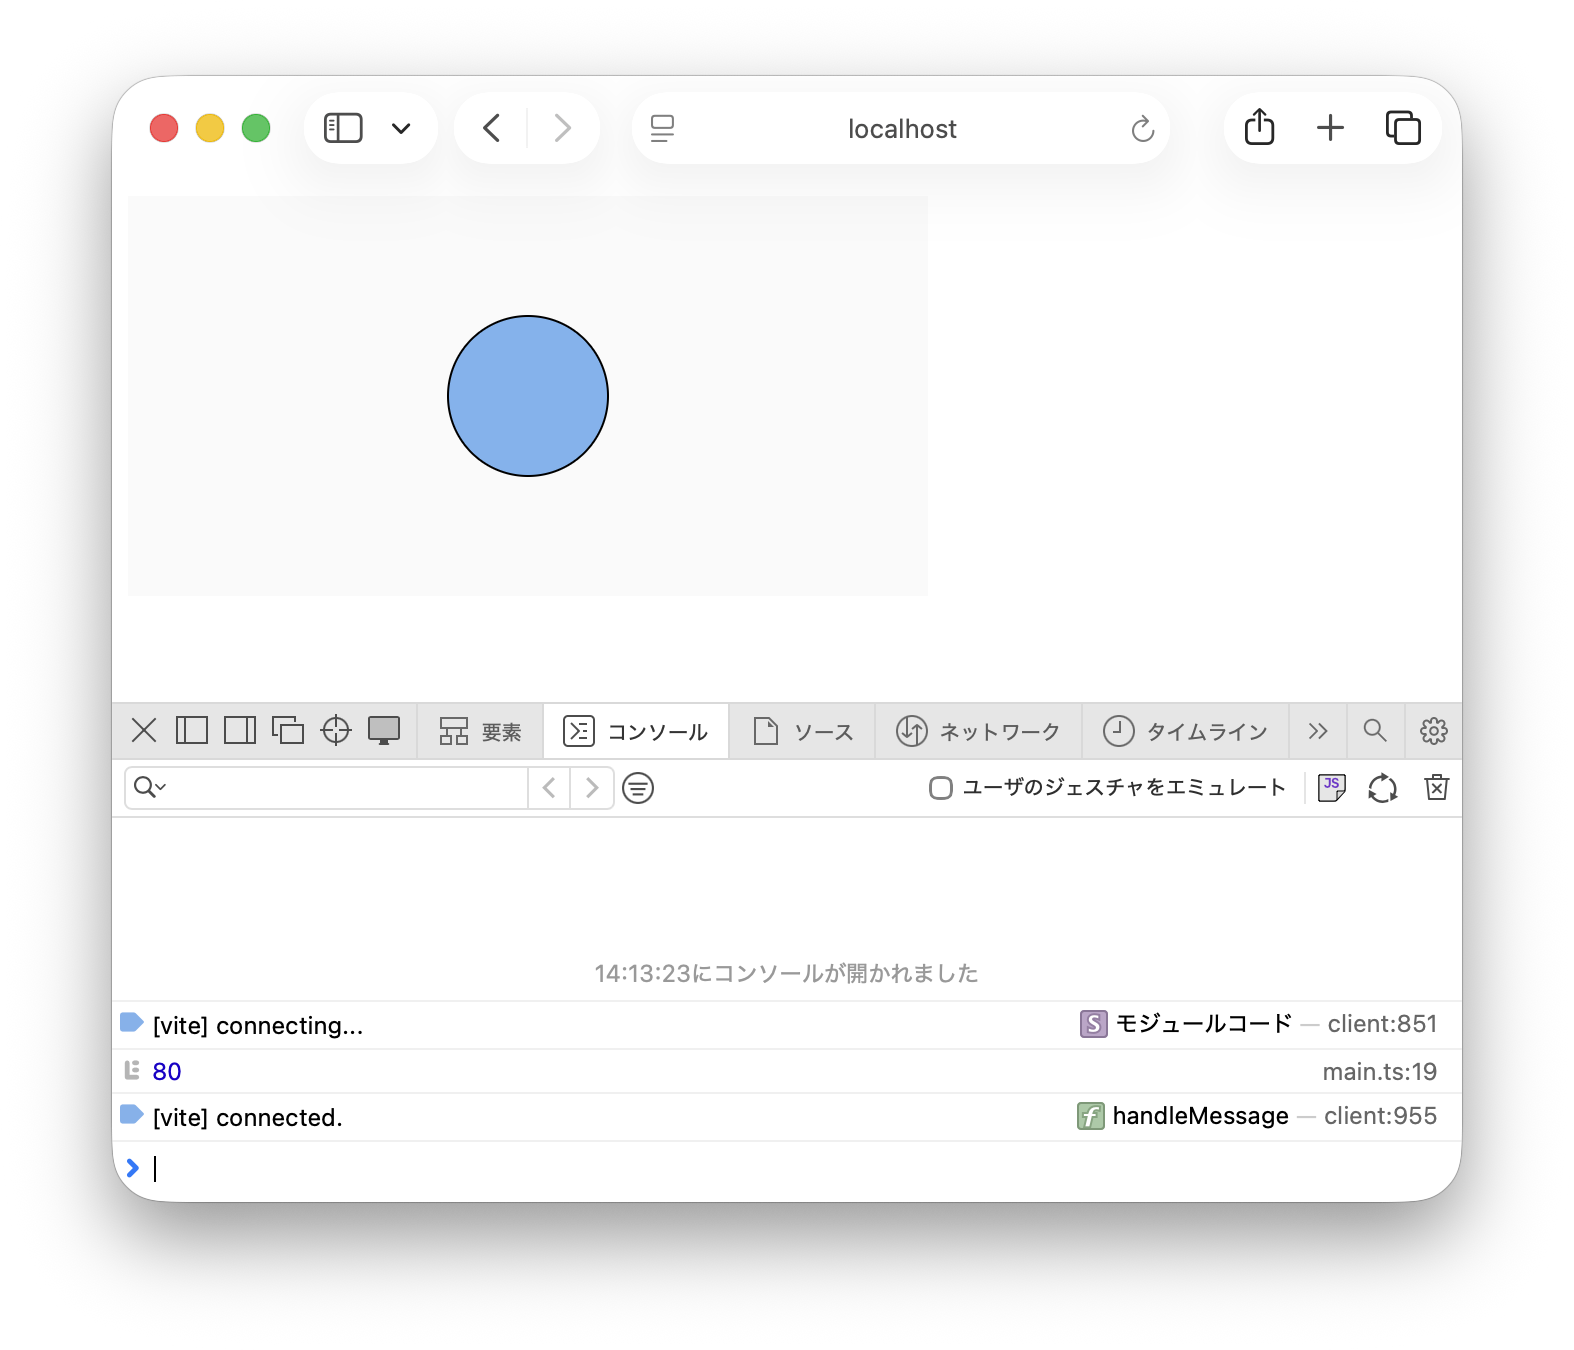
\includegraphics[width=0.6\textwidth]{figures/chapter04/console-value.png}
    \caption{ブラウザの開発者ツールのコンソールに表示された値}
    \label{fig:chapter04-console-value}
\end{figure}

自分の使っているブラウザで、\texttt{console.log}で出力されたものを見る方法を確認しておいて下さい。

\section{円弧を描く}

円や楕円の一部分だけを描きたいときには、\texttt{arc}関数を使います。
\texttt{arc}関数は角度を指定するため、少しだけ新しい考え方が入ります。
ここでは詳しい角度の計算には踏み込まず、口が開いた円のような形を描くための命令として使ってみます。

\begin{listing}[htbp]
\inputminted{ts}{listings/chapter04/arc-pacman.ts}
\caption{arcで口が開いた円を描く}
\label{lst:chapter04-arc-pacman}
\end{listing}

\texttt{p.arc}の最初の4つの数値は、\texttt{p.ellipse}と同じように、中心の位置、幅、高さを表します。その後ろに、描き始める角度と描き終わる角度を指定します。このサンプルでは、\texttt{startAngle}と\texttt{endAngle}という変数を使い、どの角度からどの角度まで描くのかを読み取りやすくしています。最後の\texttt{p.PIE}は、円弧の両端を中心と結び、扇形のように描くための指定です。

\begin{figure}[htbp]
    \centering
    \begin{tikzpicture}[x=1cm, y=-1cm, font=\small]
        \tikzset{
            guide/.style={draw=black!35, dashed, line width=0.6pt},
            arrow/.style={->, line width=0.7pt},
            measure/.style={<->, line width=0.7pt},
            arcline/.style={draw=orange!80!black, fill=yellow!60, line width=1pt},
            labelbox/.style={
                draw=black!35,
                fill=white,
                rounded corners=2pt,
                inner xsep=5pt,
                inner ysep=3pt,
                align=center
            }
        }

        \coordinate (center) at (0,0);
        \coordinate (start) at ({2.5*cos(45)},{1.5*sin(45)});
        \coordinate (end) at ({2.5*cos(315)},{1.5*sin(315)});

        \draw[guide] (-2.5,-1.5) rectangle (2.5,1.5);
        \draw[guide] (center) ellipse (2.5 and 1.5);
        \path[arcline]
            (start)
            plot[domain=45:315, samples=90]
                ({2.5*cos(\x)}, {1.5*sin(\x)})
            -- (center) -- cycle;
        \fill (center) circle (2pt);
        \node[labelbox, anchor=west] at (0.25,0.15) {中心\\\texttt{(x, y)}};

        \draw[measure] (-2.5,2.05) -- node[below] {\texttt{w}} (2.5,2.05);
        \draw[measure] (-3.05,-1.5) -- node[left] {\texttt{h}} (-3.05,1.5);

        \draw[arrow, red!70!black] (center) -- (start);
        \draw[arrow, blue!70!black] (center) -- (end);
        \node[labelbox, anchor=west] at (2.0,1.1) {\texttt{startAngle}\\\texttt{p.QUARTER\_PI}};
        \node[labelbox, anchor=west] at (2.0,-1.1) {\texttt{endAngle}\\\texttt{p.TWO\_PI - p.QUARTER\_PI}};

        \draw[arrow] (3.7,0) arc[start angle=0, end angle=70, radius=0.7];
        \node[anchor=west, align=left] at (4.0,0.9) {角度は右向きから\\時計回りに増える};

        \node[align=center, font=\ttfamily\small] at (0,2.9)
            {p.arc(x, y, w, h, startAngle, endAngle, p.PIE)};
    \end{tikzpicture}
    \caption{\texttt{arc}関数の引数と円弧の関係}
    \label{fig:chapter04-arc-arguments}
\end{figure}

p5.jsでは、標準では角度をラジアンという単位で表します。
学校でよく使う90度、180度、360度のような表し方とは違いますが、
円を一周する角度を\texttt{p.TWO\_PI}$=2\pi$と考えると、最初は扱いやすくなります。
p5.jsの画面では、右向きが\texttt{0}で、そこから時計回りに角度が増えていきます。
そのため、下向きが\texttt{p.HALF\_PI}$=\frac{\pi}{2}$、
左向きが\texttt{p.PI}$=\pi$、
一周して右向きに戻る角度が\texttt{p.TWO\_PI}$=2\pi$になります（図\ref{fig:chapter04-p5-angle-directions}参照）。

\begin{figure}[htbp]
    \centering
    \begin{tikzpicture}[x=1cm, y=-1cm, font=\small]
        \tikzset{
            axis/.style={->, draw=black!45, line width=0.7pt},
            guide/.style={draw=black!30, dashed, line width=0.5pt},
            anglearrow/.style={->, draw=orange!80!black, line width=1.2pt},
            pointlabel/.style={
                draw=black!35,
                fill=white,
                rounded corners=2pt,
                inner xsep=5pt,
                inner ysep=3pt,
                align=center
            }
        }

        \coordinate (center) at (0,0);
        \draw[guide] (center) circle (2.0);
        \draw[axis] (-2.55,0) -- (2.8,0) node[right] {$x$};
        \draw[axis] (0,-2.55) -- (0,2.8) node[below] {$y$};
        \fill (center) circle (2pt);

        \draw[anglearrow]
            (1.05,0)
            arc[start angle=0, end angle=90, radius=1.05];
        \node[align=center] at (1.65,0.75) {角度は\\時計回り};

        \fill (2.0,0) circle (2pt);
        \fill (0,2.0) circle (2pt);
        \fill (-2.0,0) circle (2pt);
        \fill (0,-2.0) circle (2pt);

        \node[pointlabel, anchor=west] at (2.25,0) {\texttt{0}\\右向き};
        \node[pointlabel, anchor=north] at (0,2.35) {\texttt{p.HALF\_PI}\\下向き};
        \node[pointlabel, anchor=east] at (-2.25,0) {\texttt{p.PI}\\左向き};
        \node[pointlabel, anchor=south] at (0,-2.35) {\texttt{p.PI + p.HALF\_PI}\\上向き};
        \node[pointlabel, anchor=west] at (2.25,1.15) {\texttt{p.TWO\_PI}\\一周して右向き};
    \end{tikzpicture}
    \caption{p5.jsにおける角度の向き}
    \label{fig:chapter04-p5-angle-directions}
\end{figure}

\section{よくある間違い}

変数を使うとプログラムは読みやすくなりますが、名前、型、代入のルールを混同するとエラーや意図しない動作の原因になります。

\begin{mistakebox}{変数名が短すぎて意味が分からない}
\texttt{x}や\texttt{d}だけでは、何を表す値なのか分かりにくいことがあります。短いサンプルでは使える場合もありますが、教材では\texttt{circleX}や\texttt{circleDiameter}のように意味が分かる名前を使います。
\end{mistakebox}

\begin{mistakebox}{同じ名前の変数をもう一度作る}
同じ場所で\texttt{const circleX: number = 100;}と書いた後、もう一度\texttt{const circleX: number = 240;}と書くことはできません。値を変えたい場合は、\texttt{let}で作ってから代入します。
\end{mistakebox}

\begin{mistakebox}{number型に文字列を入れる}
\texttt{const circleX: number = "100";}のように、\texttt{number}型の変数に文字列を入れることはできません。数字として使う値は、引用符で囲まずに書きます。
\end{mistakebox}

\begin{mistakebox}{p.widthのp.を付け忘れる}
instance modeでは、\texttt{width}ではなく\texttt{p.width}と書きます。\texttt{height}、\texttt{mouseX}、\texttt{mouseY}なども同じように\texttt{p.}を付けます。
\end{mistakebox}

\begin{mistakebox}{arcの角度を普通の度数だと思う}
\texttt{p.arc}の角度は、90度や180度のような度数ではなく、ラジアンで指定します。最初は\texttt{p.QUARTER\_PI}、\texttt{p.PI}、\texttt{p.TWO\_PI}のような用意された値を使うと分かりやすいです。
\end{mistakebox}

\section{まとめ}

この章では、変数と型注釈を使って、数値に意味のある名前を付ける方法を学びました。\texttt{const}は変わらない値、\texttt{let}は後から変える値に使います。数値を表す型注釈として、\texttt{: number}を書きます。

また、変数を使って計算式を書いたり、\texttt{p.width}や\texttt{p.height}からキャンバスの大きさを利用したりする方法も確認しました。最後に、\texttt{p.arc}で円の一部を描き、角度にも名前を付けられることを見ました。変数を使う目的は、単に短く書くことではなく、プログラムの意味を読みやすくすることです。

\section{演習問題}

この章の演習では、直接書いていた数値を変数に置き換えながら、型注釈と変数名の付け方に慣れていきます。最初はサンプルの一部を変更し、最後は自分の図形作品を変数で整理してみましょう。

\begin{enumerate}
    \item \texttt{circleDiameter}の値を変えて、3つの円の大きさをまとめて変えてください。
    \item \texttt{circleY}の値を変えて、3つの円を上や下に移動してください。
    \item \texttt{const}で背景の明るさを表す\texttt{backgroundGray}を作り、\texttt{p.background}で使ってください。
    \item \texttt{let circleX: number}を使い、同じ変数の値を変えながら4つの円を横に並べてください。
    \item \texttt{circleSpacing}の値を変えて、円どうしの間隔を広くしたり狭くしたりしてください。
    \item \texttt{p.width / 2}と\texttt{p.height / 2}を使い、キャンバスの中央に長方形を描いてください。
    \item \texttt{circleRadius}から\texttt{circleDiameter}を計算し、その直径で円を描いてください。
    \item 第3章で作った色付きの顔のサンプル\ref{lst:chapter03-color-state}で、顔の中心座標や目の直径を変数にしてください。
    \item \texttt{console.log}を使い、計算した直径や中央座標の値を確認してください。
    \item \texttt{p.arc}を使い、口の開き方が違う円を2つ描いてください。
    \item 挑戦問題として、家、ロボット、パックマン風のキャラクターなどを作り、位置、大きさ、色、角度の数値を分かりやすい変数名で整理してください。
\end{enumerate}
